\chapter{Experiments and Evaluation}
\label{ch:experiments}

This chapter evaluates the four method stages through one evaluation setup and three experiments. Stage 1 establishes the experimental dataset, reference records, and data partitions used in the evaluation. Experiment I evaluates the three building attributes predicted in Stage 2. Experiment II evaluates the archetype cells and thermal parameters produced in Stage 3. Experiment III compares the energy class prediction procedures implemented in Stage 4. The Experimental Design and Results sections follow the same experiment order, creating a direct link between every comparison, metric, and reported result. The chapter closes with a discussion of the findings, their relation to prior work, and the limits of the evidence.

\section{Experimental Design}
\label{sec:strategy_metrics}

The experimental design first defines the evaluation setup and then presents the three experiments aligned with the research objectives. Table~\ref{tab:experiment_correspondence} defines the role of each component and its matching Results subsection. The dataset checks establish the data composition and target conditions under which all results are interpreted. Experiments I, II, and III then follow the information flow from building attributes predicted from images to archetype assignment and energy class prediction.

\begin{table}[htbp]
	\centering
	\caption{Correspondence between method stages, experiments, evidence, and Results subsections.}
	\label{tab:experiment_correspondence}
	\footnotesize
	\begin{tblr}{
		width = \linewidth,
		colspec = {Q[l,m,1.8cm] Q[l,m,2.2cm] X[l] X[l] Q[l,m,2.4cm]},
		colsep = 3pt,
		row{1} = {font=\bfseries},
		rowsep = 2pt,
	}
		\toprule
		Component & Method stage & Evaluation question & Principal evidence & Results subsection \\
		\midrule
		Evaluation setup & Stage 1 & Which buildings and reference targets support the three experiments? & Building and image counts, dataset composition, and certificate consistency & Dataset Composition and Target Consistency \\
		Experiment I & Stage 2 & How accurately can the three vision configurations predict building type, construction year, and floor count? & Classification and regression metrics on the evaluation set & Building Attribute Prediction \\
		Experiment II & Stage 3 & How do errors in predicted type and year affect the assigned archetype cell and thermal parameters? & Joint cell metrics and $h_{tr}$ differences & Archetype Assignment and Thermal Consequences \\
		Experiment III & Stage 4 & How does the source of building information affect energy class prediction? & Binary and seven-class comparisons and feature ablation & Energy Class Prediction \\
		\bottomrule
	\end{tblr}
\end{table}

\subsection{Evaluation Setup}
\label{sec:dataset_statistics}

The experimental dataset contains 10,086 buildings and 47,150 images. A predefined building-level partition assigns 8,068 buildings to the development set and 2,018 to the fixed holdout set. All images associated with one building remain within the same partition.

All holdout performance comparisons in Experiments I to III are calculated on an evaluation set of 2,014 buildings. Two holdout buildings are excluded because InternVL3-2B did not return complete predictions for building type, construction year, and floor count, and two are excluded because their reconstructed areas did not satisfy the validity criteria for the thermal calculation. Appendix~\ref{sec:appendix_a_evaluation_set} reports the excluded records and the corresponding validity criteria.

\subsection{Experiment I: Building Attribute Prediction}
\label{sec:prediction_tasks_metrics}

Experiment I first quantifies the accuracy of the predicted building attributes, which serve as inputs to the subsequent archetype assignment and energy calculation stages. ResNet-50 with full fine tuning, DINOv2 with a frozen backbone and trained prediction heads, and InternVL3-2B without parameter updating are evaluated on the same 2,014 buildings. Each configuration predicts building type, construction year, and floor count. 

\paragraph{E1a: Building type.}
Building type is a four-class prediction task covering Single Family House (SFH), Terraced House (TH), Multi Family House (MFH), and Apartment Block (AB). Macro F1 is the principal metric because it gives equal weight to each class. Accuracy is reported as a complementary metric, while class recall and the confusion matrix reveal whether a high aggregate value is concentrated in the dominant AB class.

\paragraph{E1b: Construction year and \acs{TABULA} period.}
Construction year is evaluated using mean absolute error (MAE) and the coefficient of determination, $R^2$. MAE reports the average error in years, while $R^2$ measures the captured variation relative to prediction of the evaluation mean. Each predicted and reference year is also mapped through the same TABULA-NL period function. Period accuracy then reports the proportion of buildings assigned to the reference construction period, because a year error affects Stage 3 only when it changes the period.

\paragraph{E1c: Floor count.}
Floor count is evaluated using MAE and $R^2$. The two metrics distinguish a small average deviation from genuine recovery of building-level variation in an evaluation set with a restricted floor count range.

\subsection{Experiment II: Archetype Assignment and Thermal Consequences}
\label{sec:weighted_archetype_metric}

Experiment II examines how prediction errors at the attribute level affect archetype assignment and the resulting thermal comparison. At the archetype level, E2a measures whether the predicted residential size class and construction period identify the reference TABULA-NL cell for each building. For the thermal comparison, E2b converts the reference and predicted cells into representative U-values and compares the resulting transmission heat transfer.

\paragraph{E2a: Joint archetype cell assignment.}
The TABULA-NL cell depends jointly on residential size class $s$ and construction period $p(y)$. Joint accuracy is therefore defined as

\begin{equation}
	\label{eq:joint_acc}
	\mathrm{JointAcc}
	= \frac{1}{n}\sum_{i=1}^{n}
	\mathbf{1}\!\left[\hat{s}_i = s_i \;\land\; p(\hat{y}_i) = p(y_i)\right].
\end{equation}

Uniform assignment across the 24 cells has an expected accuracy of $1/24 \approx 0.042$. A second baseline assigns every building to the most frequent reference cell. Macro cell recall is also reported as the unweighted mean recall across occupied cells. Joint accuracy measures overall agreement, while macro cell recall reveals performance outside the dominant cells.

\paragraph{E2b: Thermal consequences of cell assignment.}
Categorical cell agreement gives equal weight to errors between thermally similar and thermally different cells. The second evaluation therefore compares the floor-area-normalised transmission heat transfer coefficient $h_{tr}$ obtained from the reference and predicted cells. The notation follows the distinction between an overall transmission heat transfer coefficient and its value per square metre of reference floor area in the \acs{TABULA} calculation method \parencite{loga2013calculation}. The comparison uses the U-values assigned by the relevant TABULA-NL cell, reconstructed 3DBAG areas, and a fixed window-to-wall ratio (WWR) of 0.25 in both calculations. Appendix~\ref{sec:appendix_c_wwr} reports the sensitivity of the comparison to alternative WWR values. Shared walls are treated as adiabatic.

For building $i$, the comparison quantity is

\begin{equation}
	\label{eq:htr}
	\begin{split}
		h_{tr,i} = \frac{1}{A_{floor,i}} \Bigl[
		 & U_{wall,i}A_{wall,i}(1-\mathrm{WWR}) + U_{window,i}A_{wall,i}\,\mathrm{WWR} \\
		 & + U_{roof,i}A_{roof,i} + U_{floor,i}A_{ground,i} \Bigr],
		 \qquad [\mathrm{W/(K\,m^2)}] .
	\end{split}
\end{equation}

The equation is evaluated twice for every building. One calculation uses U-values from the reference cell and the other uses U-values from the predicted cell; reconstructed areas and WWR remain fixed. Agreement is evaluated using MAE and

\begin{equation}
	\label{eq:htr_r2}
	R^2_{h_{tr}}
	= 1 - \frac{\sum_i\left(h_{tr,\mathrm{pred},i} - h_{tr,\mathrm{ref},i}\right)^2}
	{\sum_i\left(h_{tr,\mathrm{ref},i} - \overline{h_{tr,\mathrm{ref}}}\right)^2}.
\end{equation}

Weighting each floor-area-normalised value by $A_{floor}$ converts it to the corresponding building-level contribution before aggregation. Dividing the aggregate difference by the reference aggregate expresses the result as a relative percentage. This study therefore defines the floor-area-weighted relative difference as

\begin{equation}
	\label{eq:area_weighted_difference}
	\Delta_{A,h_{tr}}
	= \frac{\sum_i h_{tr,\mathrm{pred},i}A_{floor,i} - \sum_i h_{tr,\mathrm{ref},i}A_{floor,i}}
	{\sum_i h_{tr,\mathrm{ref},i}A_{floor,i}} .
\end{equation}

A positive value means that cells assigned from image predictions produce a larger aggregate transmission heat transfer coefficient than cells assigned from reference attributes, while a negative value means the opposite. The metric compares two archetype assignments and is not a validation against measured heat loss or energy use. Table~\ref{tab:htr_inputs} summarises the quantities that vary between the reference and predicted cell calculations and those held constant.

\begin{table}[htbp]
	\centering
	\caption{Inputs and data sources for calculating $h_{tr}$.}
	\label{tab:htr_inputs}
	\footnotesize
	\begin{tblr}{
		width = \linewidth,
		colspec = {Q[l,m,2.5cm] X[l] X[l] X[l]},
		colsep = 3pt,
		row{1} = {font=\bfseries},
		rowsep = 2pt,
	}
		\toprule
		Symbol & Quantity & Source & Role in the comparison \\
		\midrule
		$U_{wall}$, $U_{roof}$, $U_{floor}$, $U_{window}$ & Envelope U-values & TABULA-NL cell lookup & Vary between the reference and predicted cells \\
		$A_{wall}$ & External facade area excluding shared walls & Reconstructed 3DBAG \acs{LoD}2.2 geometry & Fixed for both calculations \\
		$A_{roof}$ & Roof area & Reconstructed 3DBAG \acs{LoD}2.2 geometry & Fixed for both calculations \\
		$A_{ground}$ & Area in contact with the ground & Reconstructed 3DBAG \acs{LoD}2.2 geometry & Fixed for both calculations \\
		$A_{floor}$ & Estimated floor area & Reconstructed 3DBAG geometry & Denominator and aggregation weight \\
		WWR & Fraction of facade area assigned to windows & Assumed value & Fixed for both calculations at each tested value \\
		\bottomrule
	\end{tblr}
\end{table}

\subsection{Experiment III: Energy Class Prediction}
\label{sec:information_source_conditions}

Experiment III compares prediction performance for the registered energy class across three input conditions: reference building attributes, predicted building attributes, and direct prediction from street view images.
 Table~\ref{tab:evaluation_conditions} defines the three energy class prediction conditions and the analytic baseline. The reference and predicted attribute conditions use the same fitted \acs{LightGBM} classifier. Their difference therefore isolates the change from reference to predicted building type, construction year, floor count, and the U-values selected by type and year. The direct image condition uses a separate image classifier and represents an alternative prediction procedure rather than an isolated input substitution.

\begin{table}[htbp]
	\centering
	\caption{Energy class prediction conditions used in Experiment III.}
	\label{tab:evaluation_conditions}
	\footnotesize
	\begin{tblr}{
		width = \linewidth,
		colspec = {Q[l,m,3.1cm] X[l] X[l]},
		colsep = 3pt,
		row{1} = {font=\bfseries},
		rowsep = 2pt,
	}
		\toprule
		Condition & Input & Prediction procedure \\
		\midrule
		Uniform random baseline & No building information & Equal prediction probability for every target class; expected metrics calculated analytically \\
		Reference attributes & Reference building type, construction year, floor count, four TABULA-NL U-values, and study area & Fixed LightGBM classifier fitted on reference inputs from the development set \\
		Predicted attributes & Predicted building type, construction year, floor count, four U-values selected by predicted type and year, and study area & Same fitted LightGBM classifier as the reference attribute condition \\
		Direct image & \ac{SVI} & Energy class head or fixed InternVL3-2B prompt applied without intermediate attributes \\
		\bottomrule
	\end{tblr}
\end{table}

\paragraph{E3a: Binary energy class prediction.}
The primary target distinguishes classes A to C from classes D to G. Separate classifiers are trained for this target rather than collapsing predictions from the seven-class task. The principal metric is macro F1 at a probability threshold of 0.5. Macro precision, macro recall, and recall for classes D to G describe performance across the two class groups.

\paragraph{E3b: Seven-class energy class prediction.}
The secondary task predicts classes A to G after ratings above A are combined with class A. Macro F1 is the principal class-balanced metric. Exact accuracy is reported for comparability with previous work, and $\pm1$ accuracy reports the proportion of predictions within one adjacent class of the registered value. Because the majority class alone attains a $\pm1$ accuracy of 0.612 on the evaluation set, this metric is interpreted only with macro F1 and both random and majority baselines.

\paragraph{E3c: Feature contribution analysis.}
A feature contribution analysis assesses the marginal contribution of each structured input to energy class prediction. Leave-one-out ablation on the development set measures the change in macro F1 when construction year, building type, floor count, the four TABULA U-values, or study area is removed from the reference input set. As a separate test, four reconstructed 3DBAG geometry features, building volume, estimated floor area, shape factor, and shared wall ratio, are added to assess whether geometric information not explicitly represented by the eight main inputs improves prediction performance. All ablation models use the same five development folds, fixed LightGBM settings, and no class weighting.

\section{Results}
\label{sec:quantitative_results}

The Results follow the order established in Table~\ref{tab:experiment_correspondence}. Dataset and target checks are reported first. Experiments I, II, and III then present the observations produced by the corresponding design.

\subsection{Dataset Composition and Target Consistency}
\label{sec:building_level_consistency}

The experimental dataset contains 10,086 buildings and 47,150 images. Table~\ref{tab:city_composition} reports the predefined development and holdout sets by study area. Amsterdam accounts for 8,011 buildings, or 79.4\% of the experimental dataset.

\begin{table}[htbp]
	\centering
	\caption{Study area composition and predefined partition of the experimental dataset.}
	\label{tab:city_composition}
	\footnotesize
	\begin{tblr}{
		width = \linewidth,
		colspec = {Q[l,m,1.9cm] X[r] X[r] X[r] X[r] X[r] X[r]},
		colsep = 3pt,
		row{1} = {font=\bfseries},
		row{Z} = {font=\bfseries},
		rowsep = 2pt,
	}
		\toprule
		Study area & Development buildings & Development images & Holdout buildings & Holdout images & Total buildings & Total images \\
		\midrule
		Amsterdam & 6,416 & 29,309 & 1,595 & 7,215 & 8,011 & 36,524 \\
		Rotterdam & 1,129 & 5,864 & 286 & 1,460 & 1,415 & 7,324 \\
		Utrecht & 384 & 1,778 & 103 & 454 & 487 & 2,232 \\
		Delft & 139 & 871 & 34 & 199 & 173 & 1,070 \\
		\midrule
		Total & 8,068 & 37,822 & 2,018 & 9,328 & 10,086 & 47,150 \\
		\bottomrule
	\end{tblr}
\end{table}

Figure~\ref{fig:svi_examples} provides one representative crop for each available combination of study area and residential building type. The missing MFH example in Delft reflects the absence of that combination from the experimental dataset.

\begin{figure}[htbp]
	\centering
	\includegraphics[width=0.85\linewidth]{figures/fig/fig_3_4_examples}
	\caption{Representative cropped street view images across the four study areas and four residential building types.}
	\label{fig:svi_examples}
\end{figure}

Figure~\ref{fig:distributions} shows the corresponding distributions of building type, floor count, construction period, and registered energy class. AB accounts for approximately 88\% of the experimental dataset, compared with approximately 54\% of the 124,784 buildings in the eligible reference set. Under the binary target, classes A to C account for 70.3\% of the experimental dataset and 76.5\% of the eligible reference set. The experimental results therefore describe buildings with at least one image meeting the Stage 1 selection rules rather than the complete residential building stock of the four study areas.

\begin{figure}[htbp]
	\centering
	\includegraphics[width=\linewidth]{figures/fig/fig_4_1_distributions}
	\caption[Composition of the experimental dataset across the four study areas.]{Composition of the 10,086 buildings in the experimental dataset across Amsterdam, Rotterdam, Utrecht, and Delft. Stacked bars report residential building type, floor count, TABULA-NL construction period, and registered energy class after ratings above A were combined with class A. Values above the bars report the number of buildings in each study area.}
	\label{fig:distributions}
\end{figure}

Certificate records were linked to all 10,086 buildings in the experimental dataset. Among these buildings, 58.4\% had multiple certificates, and 77.1\% of this group had more than one registered energy class. For 88.0\% of buildings, the class from the most recent certificate matched the modal class across all linked certificates. Table~\ref{tab:class_consistency} summarises these checks.

\begin{table}[htbp]
	\centering
	\caption{Consistency of energy classes across certificate records in the experimental dataset ($n=10{,}086$ buildings).}
	\label{tab:class_consistency}
	\small
	\begin{tblr}{
		width = \linewidth,
		colspec = {X[l] Q[r,m,4.6cm]},
		colsep = 4pt,
		row{1} = {font=\bfseries},
		rowsep = 2pt,
	}
		\toprule
		Measure & Value \\
		\midrule
		Buildings linked to multiple certificates & 58.4\% \\
		Multiple-certificate buildings with inconsistent energy classes & 77.1\% \\
		Buildings whose selected latest class matched the modal class & 88.0\% \\
		\bottomrule
	\end{tblr}
\end{table}

\subsection{Experiment I Results: Building Attribute Prediction}
\label{sec:upstream_attribute_extraction}

Experiment I compares the three vision configurations for all three attributes. Table~\ref{tab:upstream_attributes} reports the principal metrics on the evaluation set. DINOv2 produced the best value in six of the seven metric columns. ResNet-50 attained the highest type accuracy, while InternVL3-2B without parameter updating performed worst on every metric.

\begin{table}[htbp]
	\centering
	\caption{Building attribute prediction on the evaluation set.}
	\label{tab:upstream_attributes}
	\footnotesize
	\begin{tblr}{
		width = \linewidth,
		colspec = {Q[l,m,2.8cm] X[r] X[r] X[r] X[r] X[r] X[r] X[r]},
		colsep = 2pt,
		row{1} = {font=\bfseries},
		rowsep = 2pt,
	}
		\toprule
		Vision configuration & Type accuracy & Type macro F1 & Year MAE & Year $R^2$ & Period accuracy & Floor MAE & Floor $R^2$ \\
		\midrule
		DINOv2, frozen backbone & 0.902 & \textbf{0.522} & \textbf{9.40} & \textbf{0.681} & \textbf{0.902} & \textbf{0.375} & \textbf{0.558} \\
		ResNet-50, full fine tuning & \textbf{0.916} & 0.495 & 11.75 & 0.551 & 0.893 & 0.425 & 0.542 \\
		InternVL3-2B, no parameter update & 0.495 & 0.246 & 30.65 & $-0.547$ & 0.769 & 0.708 & 0.010 \\
		\bottomrule
	\end{tblr}
	\par\vspace{0.4em}
	\begin{minipage}{\linewidth}
		\footnotesize\textit{Note.} All metrics are computed on the 2,014-building evaluation set. Year MAE is reported in years and floor MAE in floors.
	\end{minipage}
\end{table}

\paragraph{E1a: Building type.}
ResNet-50 and DINOv2 differed by 0.014 in accuracy but their ordering reversed for macro F1. Figure~\ref{fig:type_confusion} shows that both configurations recalled more than 0.92 of the AB buildings and none of the 12 MFH buildings. DINOv2 recalled 0.774 of TH and 0.560 of SFH, while ResNet-50 recalled 0.711 and 0.320. Because AB accounted for approximately 88\% of the evaluation set, the high accuracy primarily reflected correct AB predictions, whereas macro F1 captured the lower performance for the less frequent classes.

\begin{figure}[htbp]
	\centering
	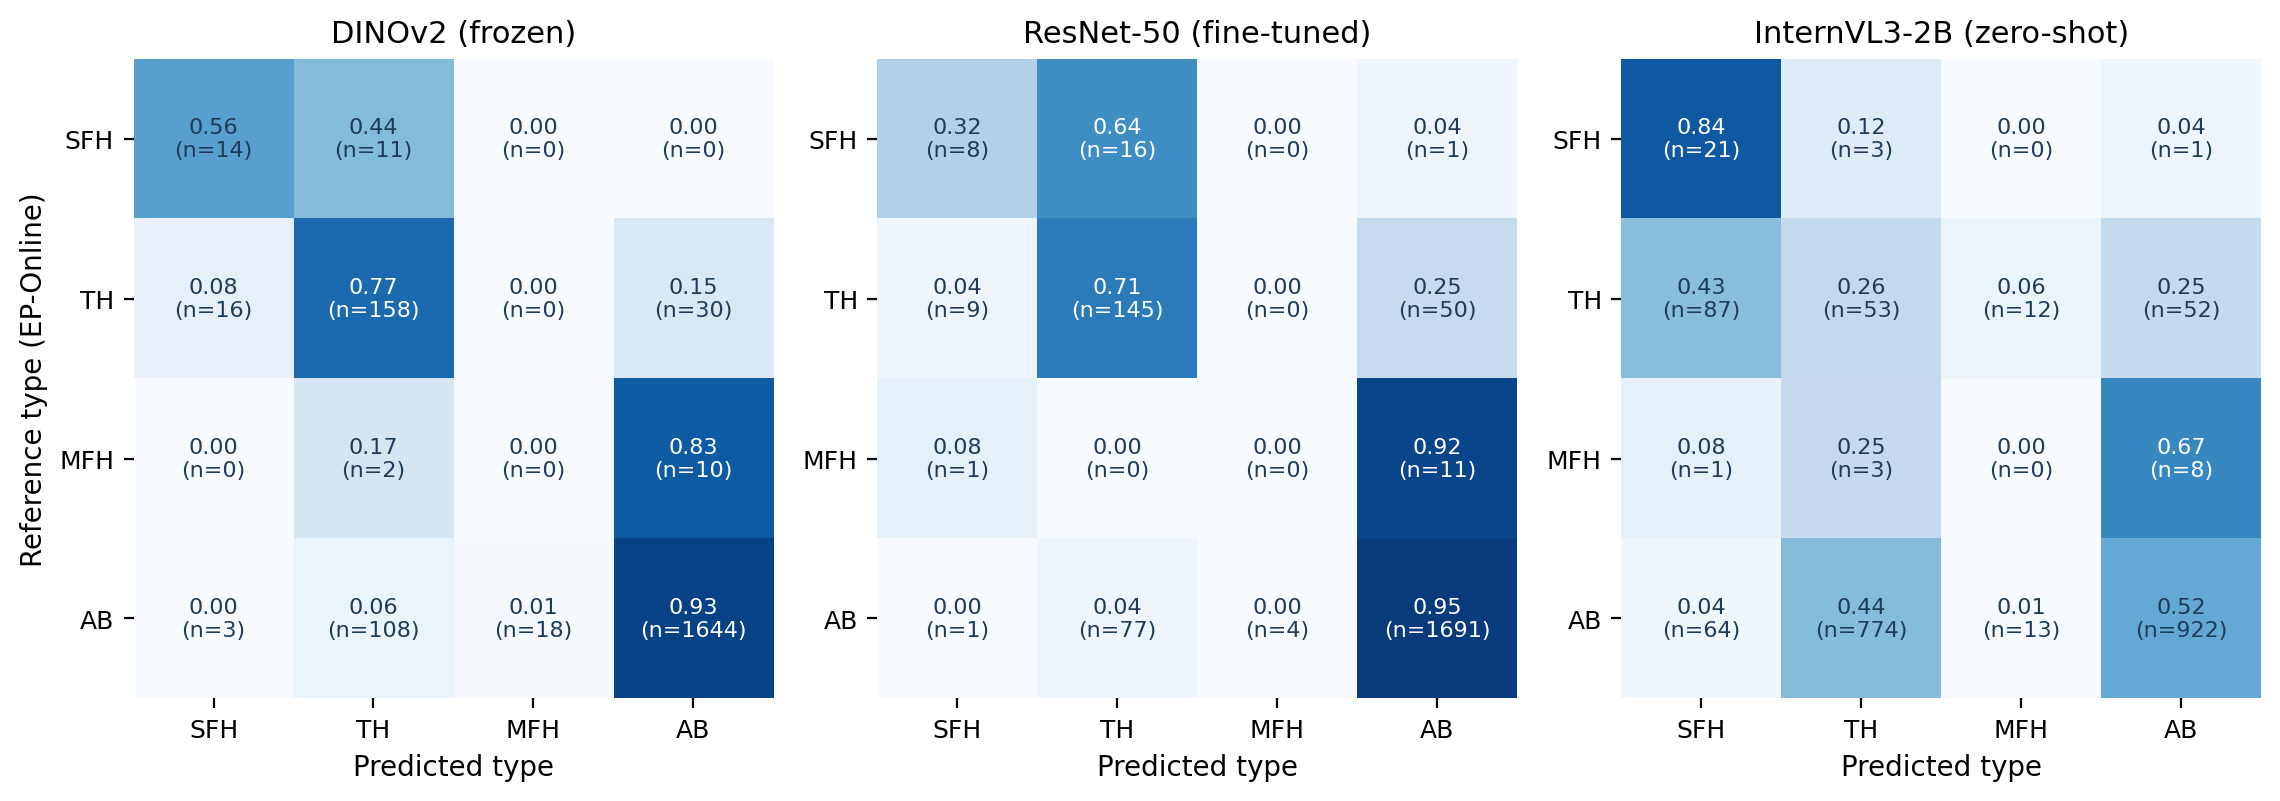
\includegraphics[width=\linewidth]{figures/fig/fig_4_2_type_confusion}
	\caption[Building type confusion matrices for the three vision configurations.]{Row-normalised building type confusion matrices for the three vision configurations on the evaluation set. Each cell also reports the number of buildings.}
	\label{fig:type_confusion}
\end{figure}

\paragraph{E1b: Construction year and \acs{TABULA} period.}
DINOv2 attained a year MAE of 9.40 years and an $R^2$ of 0.681, compared with 11.75 years and 0.551 for ResNet-50. InternVL3-2B had a year MAE of 30.65 years and a negative $R^2$. After mapping years to the six TABULA-NL periods, the corresponding period accuracies were 0.902, 0.893, and 0.769. Figure~\ref{fig:year_floor_scatter} shows that the largest deviations for the trained configurations occurred among newer buildings, whose predicted years were often earlier than their reference years.

\paragraph{E1c: Floor count.}
Floor count MAE was 0.375 for DINOv2, 0.425 for ResNet-50, and 0.708 for InternVL3-2B. Their $R^2$ values were 0.558, 0.542, and 0.010, respectively. The reference floor counts were concentrated between two and six, as shown in Figure~\ref{fig:year_floor_scatter}.

\begin{figure}[htbp]
	\centering
	\includegraphics[width=\linewidth]{figures/fig/fig_4_4_pred_vs_true_r2}
	\caption[Predicted and reference construction year and floor count.]{Predicted and reference construction year and floor count. Columns show DINOv2, ResNet-50, and InternVL3-2B; each panel reports MAE and $R^2$ on the evaluation set.}
	\label{fig:year_floor_scatter}
\end{figure}

Figure~\ref{fig:attribute_examples} presents six examples from the evaluation set to illustrate how the three vision configurations performed under different viewing conditions.
DINOv2 and ResNet-50 correctly predicted building type in the examples with partial occlusion and a distorted view. In contrast, all three configurations predicted an incorrect construction period for the examples with low image quality, a distorted view, and full occlusion. InternVL3-2B misclassified building type in one example with a clear view. Together, these cases show that correct predictions for one output did not ensure correct predictions for the others under the same viewing condition.

\begin{figure}[p]
	\centering
	\includegraphics[width=\linewidth]{../Thesis_reports/fig_ch4_svi_examples.png}
	\caption[Examples of attribute predictions under different image conditions.]{Selected examples from the evaluation set showing reference attributes and predictions from DINOv2, ResNet-50, and InternVL3-2B. Check marks indicate agreement in building type and \acs{TABULA} construction period. The examples illustrate clear views, occlusion, low image quality, and oblique viewpoints.}
	\label{fig:attribute_examples}
\end{figure}

\subsection{Experiment II Results: Archetype Assignment and Thermal Consequences}
\label{sec:joint_cell_assignment}

\paragraph{E2a: Joint archetype cell assignment.}
Table~\ref{tab:joint_cell} reports the joint cell results. DINOv2 and ResNet-50 reached joint accuracies of 0.826 and 0.827. The uniform expectation was 0.042, but the majority cell baseline was 0.791 because 1,594 of the 2,014 evaluated buildings occupied AB\,\textbar\,NL.01. Both trained configurations therefore exceeded the majority cell baseline by 0.035. InternVL3-2B reached 0.342.

\begin{table}[htbp]
	\centering
	\caption{Joint TABULA-NL cell assignment on the evaluation set.}
	\label{tab:joint_cell}
	\small
	\begin{tblr}{
		width = \linewidth,
		colspec = {X[l] Q[r,m,3.0cm] Q[r,m,3.4cm]},
		colsep = 4pt,
		row{1} = {font=\bfseries},
		rowsep = 2pt,
	}
		\toprule
		Vision configuration & Joint accuracy & Macro cell recall \\
		\midrule
		DINOv2, frozen backbone & 0.826 & \textbf{0.189} \\
		ResNet-50, full fine tuning & \textbf{0.827} & 0.135 \\
		InternVL3-2B, no parameter update & 0.342 & 0.168 \\
		\bottomrule
	\end{tblr}
	\par\vspace{0.4em}
	\begin{minipage}{\linewidth}
		\footnotesize\textit{Note.} All metrics are computed on the 2,014-building evaluation set. Expected uniform accuracy is 0.042. Majority cell accuracy is 0.791.
	\end{minipage}
\end{table}

Macro cell recall was 0.189 for DINOv2, 0.135 for ResNet-50, and 0.168 for InternVL3-2B. Figure~\ref{fig:cell_recall} shows that DINOv2 recalled 0.932 of AB\,\textbar\,NL.01 and 0.789 of TH\,\textbar\,NL.01, while recall for most cells after 1964 did not exceed 0.25. All MFH cells had zero recall. InternVL3-2B recovered some cells with one or two observations, which increased its macro cell recall despite its lower joint accuracy.

\begin{figure}[htbp]
	\centering
	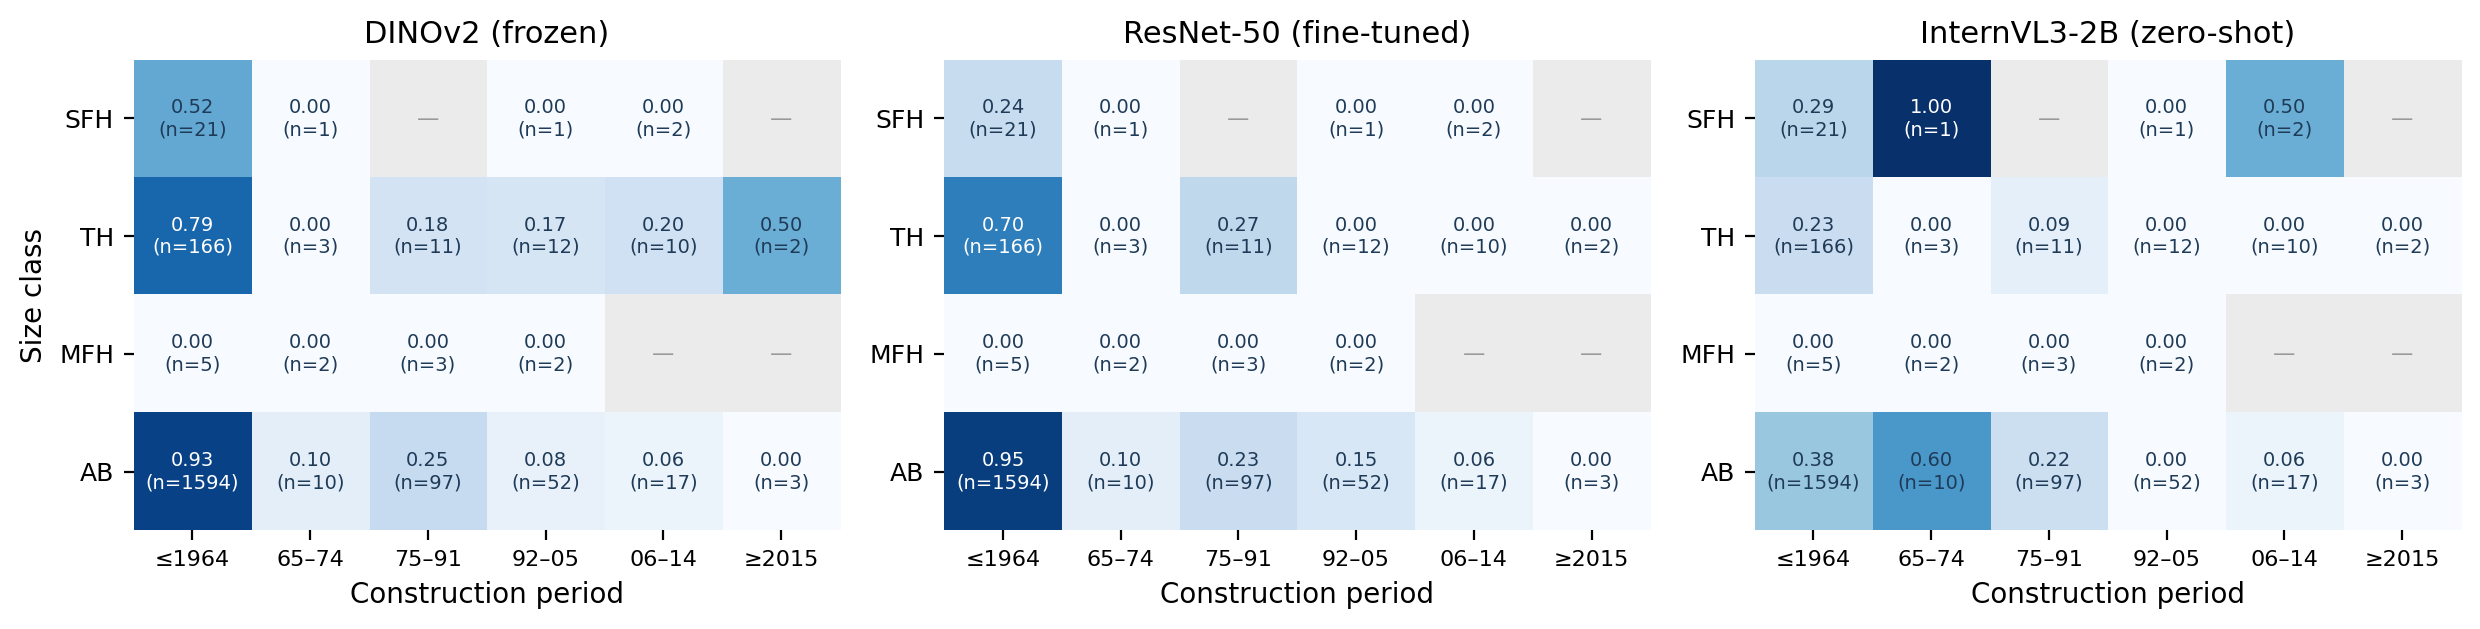
\includegraphics[width=\linewidth]{figures/fig/fig_4_3_cell_recall_heatmap}
	\caption[Recall across occupied TABULA-NL cells.]{Recall across occupied TABULA-NL cells in the evaluation set. Each cell reports recall and the number of reference buildings; cells without observations are grey.}
	\label{fig:cell_recall}
\end{figure}

\paragraph{E2b: Thermal consequences of cell assignment.}
Table~\ref{tab:htr_metrics} reports the difference between $h_{tr}$ values calculated from predicted and reference cells at $\mathrm{WWR}=0.25$. DINOv2 had an MAE of 0.149\,$\mathrm{W/(K\,m^2)}$ and an $R^2$ of 0.810. The corresponding values were 0.155 and 0.775 for ResNet-50, and 0.474 and 0.439 for InternVL3-2B. The separation in MAE between DINOv2 and InternVL3-2B was a factor of 3.2.

\begin{table}[htbp]
	\centering
	\caption{Thermal consequences of predicted archetype cells at $\mathrm{WWR}=0.25$.}
	\label{tab:htr_metrics}
	\footnotesize
	\begin{tblr}{
		width = \linewidth,
		colspec = {X[l] Q[r,m,3.0cm] Q[r,m,2.0cm] Q[r,m,3.0cm]},
		colsep = 3pt,
		row{1} = {font=\bfseries},
		rowsep = 2pt,
	}
		\toprule
		Vision configuration & $h_{tr}$ MAE ($\mathrm{W/(K\,m^2)}$) & $h_{tr}$ $R^2$ & Floor-area-weighted relative difference \\
		\midrule
		DINOv2, frozen backbone & \textbf{0.149} & \textbf{0.810} & $+9.8$\% \\
		ResNet-50, full fine tuning & 0.155 & 0.775 & $+10.2$\% \\
		InternVL3-2B, no parameter update & 0.474 & 0.439 & $+16.6$\% \\
		\bottomrule
	\end{tblr}
	\par\vspace{0.4em}
	\begin{minipage}{\linewidth}
		\footnotesize\textit{Note.} All metrics are computed on the 2,014-building evaluation set.
	\end{minipage}
\end{table}

All three configurations produced a positive floor-area-weighted relative difference from the reference cell calculations. The values ranged from $+9.8$\% for DINOv2 to $+16.6$\% for InternVL3-2B. Repeating the calculation at WWR values of 0.15, 0.25, and 0.35 left the ranking unchanged. The DINOv2 and ResNet-50 MAEs were 0.149 and 0.155 at all three WWR values at the reported precision, while the InternVL3-2B MAE changed from 0.495 to 0.453. Table~\ref{tab:wwr_sensitivity} reports the complete sensitivity results.

Experiment II therefore shows that similar overall joint accuracy for the two trained configurations corresponded to similar thermal differences, while the lower InternVL3-2B joint accuracy coincided with a substantially larger $h_{tr}$ difference.

\subsection{Experiment III Results: Energy Class Prediction}
\label{sec:energy_class_condition_comparison}

Experiment III compares all energy class prediction conditions on the 2,014-building evaluation set. Results for the primary binary target are presented first, followed by the seven-class target and feature contribution analysis.

\paragraph{E3a: Binary energy class prediction.}
Table~\ref{tab:binary_conditions} reports the default threshold results. Direct image prediction with DINOv2 attained the highest macro F1 at 0.597 and the highest macro recall at 0.601. Direct image prediction with ResNet-50 followed with a macro F1 of 0.566. The reference attribute condition reached 0.492, while predicted attributes from DINOv2 and ResNet-50 reached 0.490 and 0.488.

\begin{table}[htbp]
	\centering
	\caption{Binary energy class prediction on the evaluation set ($n=2{,}014$).}
	\label{tab:binary_conditions}
	\footnotesize
	\begin{tblr}{
		width = \linewidth,
		colspec = {Q[l,m,3.0cm] X[l] Q[r,m,1.9cm] Q[r,m,1.7cm] Q[r,m,1.5cm]},
		colsep = 3pt,
		row{1} = {font=\bfseries},
		rowsep = 2pt,
	}
		\toprule
		Condition & Vision configuration & Macro precision & Macro recall & Macro F1 \\
		\midrule
		Uniform random & Analytic expectation & 0.500 & 0.500 & 0.479 \\
		Reference attributes & LightGBM & \textbf{0.612} & 0.529 & 0.492 \\
		Direct image & DINOv2 & 0.595 & \textbf{0.601} & \textbf{0.597} \\
		Direct image & ResNet-50 & 0.566 & 0.566 & 0.566 \\
		Direct image & InternVL3-2B & 0.149 & 0.500 & 0.230 \\
		Predicted attributes & DINOv2 & 0.566 & 0.522 & 0.490 \\
		Predicted attributes & ResNet-50 & 0.550 & 0.518 & 0.488 \\
		Predicted attributes & InternVL3-2B & 0.527 & 0.528 & 0.527 \\
		\bottomrule
	\end{tblr}
\end{table}

The reference attribute condition recalled 96.0\% of classes A to C but 9.8\% of classes D to G. Predicted attributes from DINOv2 and ResNet-50 produced similar recalls of 10.8\% and 11.0\% for classes D to G. Direct DINOv2 increased recall for this group to 46.9\%. Direct InternVL3-2B assigned every building to classes D to G, so its macro F1 of 0.230 reflected a constant prediction rather than discrimination among buildings. Table~\ref{tab:binary_perclass} reports precision, recall, and F1 for both class groups.

\paragraph{E3b: Seven-class energy prediction.}
Table~\ref{tab:sevenclass_conditions} reports results for classes A to G. Direct DINOv2 attained the highest macro F1 at 0.213, followed by direct ResNet-50 at 0.201. The reference attribute condition reached 0.171 and the three predicted attribute conditions ranged from 0.131 to 0.151. The metric ranking differed for exact and $\pm1$ accuracy, for which the reference attribute condition attained the highest values of 0.358 and 0.660.

\begin{table}[htbp]
	\centering
	\caption{Seven-class energy class prediction on the evaluation set ($n=2{,}014$).}
	\label{tab:sevenclass_conditions}
	\small
	\begin{tblr}{
		width = \linewidth,
		colspec = {X[l] X[l] Q[r,m,2.1cm] Q[r,m,2.1cm] Q[r,m,2.1cm]},
		colsep = 4pt,
		row{1} = {font=\bfseries},
		rowsep = 2pt,
	}
		\toprule
		Condition & Vision configuration & Macro F1 & Exact accuracy & $\pm1$ accuracy \\
		\midrule
		Uniform random & Analytic expectation & 0.127 & 0.143 & 0.390 \\
		Reference attributes & LightGBM & 0.171 & \textbf{0.358} & \textbf{0.660} \\
		Direct image & DINOv2 & \textbf{0.213} & 0.266 & 0.544 \\
		Direct image & ResNet-50 & 0.201 & 0.263 & 0.570 \\
		Direct image & InternVL3-2B & 0.015 & 0.046 & 0.167 \\
		Predicted attributes & DINOv2 & 0.151 & 0.297 & 0.589 \\
		Predicted attributes & ResNet-50 & 0.148 & 0.284 & 0.588 \\
		Predicted attributes & InternVL3-2B & 0.131 & 0.277 & 0.596 \\
		\bottomrule
	\end{tblr}
\end{table}

Only the reference attribute condition exceeded the majority baseline of 0.612 for $\pm1$ accuracy. Direct InternVL3-2B predicted class F for approximately 99\% of the evaluation set and consequently remained below the uniform expectation for all three seven-class metrics. These results close the main comparison by showing that condition ranking depends on both target resolution and evaluation metric.

\paragraph{E3c: Feature contribution analysis.}
The leave-one-out results in Table~\ref{tab:feature_ablation} identify construction year as the largest contributor among the eight inputs of the reference attribute classifier. Removing year reduced macro F1 by 0.032 for the seven-class target and 0.030 for the binary target. Removing the four TABULA U-values changed macro F1 by less than 0.003 in either target. Adding all four clean reconstructed geometry features increased macro F1 by 0.039 for the seven-class target and 0.104 for the binary target.

\begin{table}[htbp]
	\centering
	\caption{Changes in development set macro F1 under feature removal and clean geometry augmentation.}
	\label{tab:feature_ablation}
	\small
	\begin{tblr}{
		width = \linewidth,
		colspec = {X[l] Q[r,m,3.7cm] Q[r,m,3.2cm]},
		colsep = 4pt,
		row{1} = {font=\bfseries},
		rowsep = 2pt,
	}
		\toprule
		Feature change & Seven-class $\Delta$ macro F1 & Binary $\Delta$ macro F1 \\
		\midrule
		Remove construction year & $\mathbf{-0.032}$ & $\mathbf{-0.030}$ \\
		Remove floor count & $-0.012$ & $-0.011$ \\
		Remove building type & $-0.003$ & $+0.003$ \\
		Remove four TABULA U-values & $-0.000$ & $+0.002$ \\
		Remove study area & $-0.009$ & $-0.006$ \\
		Add reconstructed shape factor & $+0.025$ & $+0.063$ \\
		Add reconstructed floor area & $+0.025$ & $+0.071$ \\
		Add all four clean 3DBAG geometry features & $+0.039$ & $+0.104$ \\
		\bottomrule
	\end{tblr}
	\par\vspace{0.4em}
	\begin{minipage}{\linewidth}
		\footnotesize\textit{Note.} The full feature baselines were 0.181 for the seven-class target and 0.478 for the binary target. Geometry additions use only reconstructed 3DBAG fields; certificate geometry fields identified by the provenance audit are excluded.
	\end{minipage}
\end{table}

Experiment III therefore yields three principal findings. Direct DINOv2 produced the highest macro F1 for both energy class targets. Replacing reference attributes with predicted building attributes changed binary macro F1 by less than 0.005 but reduced seven-class macro F1 by approximately 0.019. The feature analysis identifies construction year as the strongest contributor among the structured inputs and shows that clean reconstructed geometry adds information not captured by the main input set.

\section{Discussion}
\label{sec:discussion}

The discussion follows the correspondence between the method stages, experiments, and Results subsections established in Table~\ref{tab:experiment_correspondence}. Experiment I interprets the accuracy and failure patterns of building attribute prediction from \Ac{SVI}. The effects of prediction errors on TABULA-NL archetype assignment and thermal parameters are examined through Experiment II. Experiment III compares registered energy class prediction across the reference attribute, predicted attribute, and direct image conditions and examines the contribution of the structured inputs.

\subsection{Building Attribute Prediction}

DINOv2 used a pretrained self-supervised backbone whose parameters remained fixed, while the MLP and three attribute heads were trained on the development data. For building type prediction, DINOv2 and ResNet-50 achieved similar accuracies of 0.902 and 0.916, respectively. However, DINOv2 achieved a slightly higher macro F1 of 0.522 than the 0.495 achieved by ResNet-50, showing better performance for the less frequent SFH and TH classes. Because only the MLP and attribute heads were updated, DINOv2 had fewer trainable parameters than the fully fine-tuned ResNet-50. This combination of stronger performance for the less frequent classes and fewer trainable parameters supports using the DINOv2 configuration to enrich missing building attributes from \Ac{SVI} when labelled development data are limited.

Construction year was the strongest continuous prediction target for DINOv2, with an $R^2$ of 0.681. This value is close to the 0.710 reported by \textcite{liang2025} for a fully fine-tuned InternVL3-2B model, but the datasets, label sources, and training procedures differ, so the values are not a direct benchmark. The negative $R^2$ of the InternVL3-2B configuration in this study instead shows that prompting without parameter updates did not recover building-level year variation among the evaluated Dutch buildings. The selected examples further suggest that visibility, occlusion, and viewpoint are relevant failure conditions, although a systematic image quality experiment would be required to quantify their effects.

\subsection{Archetype Assignment and Thermal Consequences}

The joint cell result requires interpretation against both baselines. Joint accuracies above 0.82 appear high relative to uniform assignment, but the majority cell alone reaches 0.791 because the evaluation set is dominated by old apartment blocks. Macro cell recall remained below 0.19 for both trained configurations, showing that their high joint accuracy did not extend evenly to less frequent combinations of building type and construction period. Earlier energy modelling studies identified building type and construction period as sources of error \parencite{dochev2020,bass2022}. Experiment II extends this evidence by quantifying how errors in attributes predicted from images change TABULA-NL cell assignment for the same buildings.

The $h_{tr}$ comparison distinguishes cell errors by their thermal consequence. It separated DINOv2 from InternVL3-2B more clearly than joint accuracy. All three predicted cell sets produced higher aggregate transmission heat transfer coefficients than the reference assignments. The construction year scatter provides a plausible explanation. Several newer buildings were assigned to earlier periods with higher representative U-values, increasing the calculated $h_{tr}$.

\subsection{Energy Class Prediction}

For the binary target, the direct image and predicted attribute conditions based on DINOv2 and ResNet-50 exceeded the uniform random expectation for all three reported metrics. Replacing reference attributes with attributes predicted by DINOv2 reduced macro precision by 0.046, from 0.612 to 0.566, while macro F1 changed by only 0.002, from 0.492 to 0.490. The ResNet-50 predicted attribute condition produced a similar macro F1 of 0.488. These small differences indicate that attributes predicted from \Ac{SVI} retained most of the binary prediction performance available from reference attributes. However, the reference and trained predicted attribute conditions recalled only around 10\% of classes D to G. 

Direct DINOv2 achieved a macro F1 of 0.597, exceeding the 0.492 obtained by the reference attribute condition. Earlier studies similarly found that \Ac{SVI} contains information associated with registered energy performance \parencite{mayer2023uk,mayer2023dk}. The higher macro F1 therefore indicates that the complete direct DINOv2 procedure captured visual cues associated with registered energy class. 

 InternVL3-2B produced the weakest building attribute results and performed poorly when applied directly to both energy class targets. These results indicate that prompt design without parameter updating did not extract reliable energy class information from the evaluated \Ac{SVI}. Further training with local images and registered energy class labels may therefore be required.

The seven-class target reveals a clearer limitation. Macro F1 remained low for every condition, indicating that none of the evaluated procedures reliably distinguished all seven registered classes. The DINOv2 predicted attribute condition reached a $\pm1$ accuracy of 0.589, which was 0.071 below the reference attribute condition. However, its $\pm1$ accuracy remained below the majority baseline of 0.612. The results therefore suggest that predictions often remained near the registered class, but adjacent energy classes could not be separated reliably.

The feature analysis helps explain the limited performance of the structured conditions. Construction year provided the largest contribution among the eight inputs, while the deterministic TABULA-NL U-values added little information once building type and construction period were included. Reconstructed geometry improved macro F1 for both targets, showing that the main structured input set omitted relevant building information. Overall, Experiment III shows that \Ac{SVI} can preserve much of the binary prediction performance through predicted attributes. 

\subsection{Validity, Limitations, and Future Evaluation}
\label{sec:validity_limitations}

The evaluated buildings limits geographic transfer. Mapillary coverage and image filtering produced a dataset dominated by Amsterdam and AB buildings, with few examples in several building types, construction periods, archetype cells, and registered energy classes. Performance may therefore reflect this distribution. Future geographic evaluation should exclude each study area from model development in turn and report the composition and class-specific performance of every target set. 

Target validity is constrained by the difference between the certificate and analysis units. EP-Online certificates refer to dwellings, whereas the analysis uses BAG buildings. Multiple certificates were linked to 58.4\% of the 10,086 buildings, and 77.1\% of this group had inconsistent registered energy classes. Selecting the most recent certificate provides one reproducible target but may represent only one dwelling or registration date. Future evaluation should compare latest and modal class targets and align certificate and image dates.

Model performance may be improved further because hyperparameters were not exhaustively optimised for each prediction target, and InternVL3-2B was evaluated without parameter updating. Future experiments should include an open-source \ac{VLM} fine-tuned on the experimental data, class imbalance treatments, calibration analysis, and systematic hyperparameter optimisation.

The archetype and thermal results describe assigned properties and their calculated thermal implications, while measured building performance lies outside the scope of this analysis. \Ac{SVI} may show visible facade or window changes but cannot verify concealed insulation, heating system upgrades, or renovations within individual units. The thermal comparison also relies on reconstructed 3DBAG geometry, a fixed WWR range, and archetype U-values rather than measured envelope properties. Future physical evaluation should incorporate verified renovation records, measured envelope properties, and independent heat demand observations. 

Overall, \Ac{SVI} can provide useful building attributes when reference building attributes are missing, and those attributes can be connected to a transparent archetype workflow. For the evaluated energy class task, however, building type, construction year, floor count, and their TABULA-NL U-values do not contain all information required for class-balanced prediction. A practical workflow should use administrative records and reconstructed geometry where they are available, use \ac{SVI} to supplement building attributes that can be inferred from visible facades.
